% ------------- introduction --------------

\section{Smartphone sensors}

% For example the Google Pixel 3 comes with an accelerometer and gyroscope called BMI160 from Bosch, a magnetometer called LIS2MDL from STMicro, and a barometer called BMP380 from Bosch.

Nowadays smartphones come with various sensors that can be used to measure environmental properties and to estimate the orientation and motion of the device and the user. Table \ref{tbl:sensors} provides an overview of common sensors built into smartphones.

In this thesis we used the accelerometer and gyroscope to form an \gls{imu} and combine it with the magnetometer to estimate the hard iron offset.

\begin{table}[h]
    \centering
    \begin{tabular}{ | l | p{10cm} | }
    \hline
    \textbf{Sensor type} & \textbf{Description} \\ \hline
    Accelerometer        & Measures the acceleration applied to the device in $m/s^2$. \\ \hline
    Gyroscope            & Measures the rate of rotation around the device's local X, Y and Z axis. All values are in $rad/s$. \\ \hline
    Magnetometer         & Measures the ambient magnetic field in the X, Y and Z axis. All values are in micro-Tesla $\mu T$. \\ \hline
    Barometer            & Measures the atmospheric pressure in $hPa$ (millibar). \\ \hline
    Lux meter            & Measures the ambient light level in SI $lux$. \\ \hline
    \end{tabular}
    \caption{Various smartphone sensors and their measurements.}
    \label{tbl:sensors}
\end{table}

% ------------- particle filter --------------

% TODO kind of late to present a figure - maybe use more figures and examples across the chapter
An illustration of a particle filter and the resampling step is shown in Figure \ref{fig:resampling}.

\begin{figure}[hbt!]
    \centering
    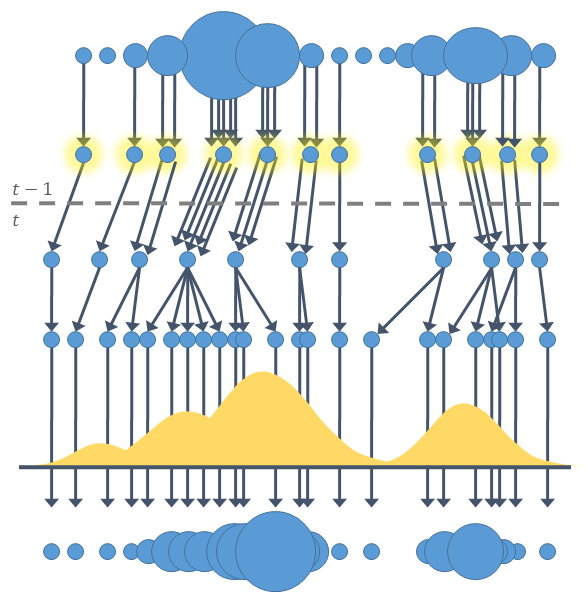
\includegraphics[width=0.6\textwidth]{figures/resampling.png}
    \caption{Illustration of the resampling step in a bootstrap particle filter. The weighted particles in the first row are replaced by equally weighted particles in the second row with similar probability density.\cite{resampling_image}}
    \label{fig:resampling}
\end{figure}

% --------------- implementation ---------------

\begin{figure}[hbt!]
    \centering
    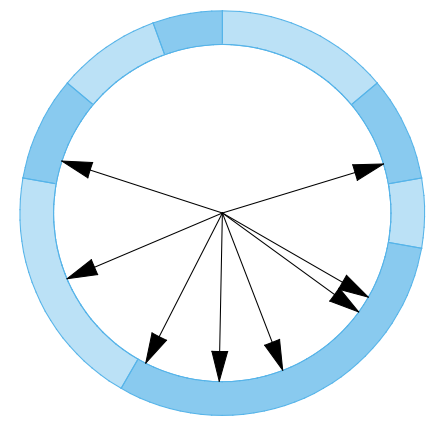
\includegraphics[width=0.2\textwidth]{figures/multinomial.png}
    \caption{Illustration of multinomial resampling with a ``resampling wheel''. The angle of the arrows are drawn from a uniform distribution across all angles.\cite{parallel_resampling}}
    \label{fig:pf_resampling}
\end{figure}
